\chapter{高通量材料设计及工作流工具的开发}\ref{chapter:workflows}
近二十年时间,计算科学逐渐开始转变为以高通量和大数据为支撑,基于大量科学数据的产生和分析处理为主要科学发现方式的学科。在这之中,高通量计算材料设计成为了材料科学分支下的一个新的重要的分支。通过将电子结构、热力学计算方法与数据挖掘和数据库技术相结合,使用当前所能达到的超级计算机的运算能力产生、计算和分析数据,科学家们能够以此来预测和指导新材料的发现与合成。该新型的材料学的研究范式的出现,使得材料的合成和发现不再单纯依赖于原本耗时耗力的大量实验,而能够在材料被发现合成之前通过计算模拟的方式来预测有价值的材料的合成。

现如今,大型计算机大大增长的计算能力和不断发展的计算方法的发展都使得计算材料学得到了长足的发展。但是,这些发展同样带来了对海量数据计算和管理的新的挑战。计算能力的发展使得高通量计算中,流程的自动化和数据量的可拓展性和易快速查询变得非常重要。同时,当数据量变得巨大,数据产生和获取过程将变得难以回溯,而这又与“可重复性”这一科学的重要原则相违背。因此,在高通量计算材料学中,为了保持1)流程自动化2)数据体量易拓展3)数据快速查询4)过程可重复等原则,科学家们开发了许多的工作流和数据库工具。

本论文的工作均使用了AiiDA\cite{pizzi2016aiida,huber2020aiida}这一工具进行计算模拟的提交和结果数据的管理查询,而且我对该工具的开发和维护也贡献了许多,将在本章后半部分介绍该工具的设计理念和应用。

\section{高通量材料设计的发展}
观察人类技术革命和社会发展个轨迹,新的社会阶段总能够与新的技术相联系。而新的技术往往又依赖于新的特定的材料。比如石器时代向青铜器时代的转变。十八世纪,以蒸汽机为技术代表的工业革命则依赖于钢铁的生产。再到今天我们所生活的,可以归功于硅芯片所主导的信息时代。而每当一种潜在材料被社会所接受,进而在后续不断的持续使用过程中发展。一段时间后,产业界将会完全转向对这种材料的依赖。大规模工业化生产线的建立,配套技术的上线和发展,无一不是在加强特定材料在社会进程中的统治地位。然而,我们很难认定人类社会在发展中所确定的某种材料就是最符合某种技术形式的材料。所以在新技术出现过程中所依赖的材料的选择和发展是一个严肃和需要反复考证的结果。而如今,材料的选择是一个涉及更为多方面的问题,新材料是否与现有的工业基础相匹配?新材料是否环境友好?新材料是否能通过成本较低原料来生产得到?而材料科学家就是要衡量和解决这样多方面多维度的问题。

在过去,材料的发现过程只能依赖于实验的合成。只有当一种材料被事实上合成,才能通过科学手段进行对材料物理化学性质的测量,进而对材料的潜在应用价值进行评估判断。因此材料的发现是一个缓慢且艰难的过程,实验科学家通过规律和经验将某种材料合成并生长成能够完整测量其性质的规模往往是一个并不简单,及其耗费时间的过程。而且,这个过程很多时候有极大的可重复性。材料和材料间很可能因为细微变量的调整而出现性质上的巨大差别。那么实验科学家则有必要全面的考察各个变量所可能导致的结果差异。而这个过程中,就存在变量以外的因素的重复。信息化工业化的今天,将人的精力耗费在不断机械重复特定流程的工作中并不是一个理想的科学模式,我们完全应该通过机械和计算机来完成对人的劳动力的解放,使得科学家的精力放在目前只有人类才能胜任的问题和工作中。那么,是否存在这样一种材料合成和发现的方式,来解放科学家的时间和双手,将重复的工作交由机械和计算机来完成,使得科学家能够着眼于问题本身的探索?而这,便是所谓的“高通量”材料设计和合成科学所期望回答的解决的问题。

高通量实验的方法最早可以追溯到约一百年前就由Edison和Ciamician\cite{ciamician1912photochemistry}所贡献的工作,到今天,高通量实验科学已经发展成更加成熟和完整的方法\cite{curtarolo2003predicting,ceder1998identification,johannesson2002combined,curtarolo2005accuracy,xiang1995combinatorial,koinuma2004combinatorial,takeuchi2003identification}。
随着计算机计算能力的发展和计算材料学方法的发展,高通量计算材料学成为一种设计的发现新型有潜在价值材料的重要方式。本论文工作主要使用和涉及了高通量计算材料学的方法和工具,将对其进行介绍。

高通量计算材料设计,顾名思义,是使用高通量的方法结合计算材料学进行材料的设计。它是计算材料学与基于数据库构建,数据挖掘的计算机技术的结合。通过对已有和理论预测的材料进行热力学、电子结构等性质的计算,之后将所否信息储存进入数据库,通过数据挖掘技术来筛选预测可能具备某种特别优秀性质的材料。因此,该技术流程的准确性,需要能够准确描述已知结构的实验性质和特征,并还需要确保使得预测的材料通过实验手段合成并表征为确实有理论预测的性质和特性。这个流程准确地符合了广义上的经验主义的科学方法论,即通过归纳来描述某类共有的科学现象并总结为规律,并且该规律还需要拥有演绎推广和预测未知的能力。只不过稍稍不同的是,在高通量计算材料设计中,归纳的过程依赖并基本完全交由计算机负责,另外,所归纳总结的规律并不是如人类总结的那样直观。但不可质疑,如果整个方法流程具备归纳演绎的效果,那么所总结的规律即便并不直观,也应该选择相信其正确性。

需要注意的是,在文献中,高通量材料研究往往会和材料性质的组合交叉测量表征、理论计算所混淆。有文献\cite{maclean1999glossary,maier2007combinatorial}试图清晰地区别这样两种研究模式,但在实际工作中并不容易区分这两者的区别。在该论文中,我们选择作如下的定义的归类,即如果实验和计算中的数据量达到人为难以处理(此处的‘人为难以处理’是一个模糊的概念),而需要且不得不借助自动化的方式进行处理的量级时,并确实通过自动化方式处理和分析的工作方式成为高通量研究方法。因此,即便数据量并不巨大,且通过人为方式耗费极大的时间能够处理,选择使用自动化处理的方式来进行替代并合理结合数据库技术,依旧认为使用了高通量的技术。

高通量材料模拟的具体实现主要分为以下三类:1)材料的模拟合成模拟生长,通过用计算材料学的方法高通量地模拟可能材料的制备和生长。2)材料信息数据库系统的建立和管理,通过合理的方式将已有材料的性质结构信息通过数据库技术合理储存,使容易查询分析而引导新的研究和发现。3)材料分类和筛选,使用数据挖掘技术对材料合成或材料特征进行分类筛选,试图得到在某些性质方面更有潜在价值的材料。其中,第三点最为有挑战性且意义重大。它需要研究人员需要对材料性质和材料特征之间的关系有深入的物理认识,从而建立一套对材料特征的合理描述符(descriptor),并在数据库中将这套描述符与目标的材料性质相关联,从而能够直观的发现材料构效间的联系,为达到预期的性能目标而容易地选择结构特征参数。描述符本身并不需要是可以实验测量的物理量,描述符应是能够联系微观参数(缺陷形成能、结构中原子所处环境、能带结构、态密度、磁矩等物理量)和材料宏观性质(湿度、延展性、临界温度等)的经验量。或者说,描述符是研究人员与数据库之间交流所使用的语言\cite{curtarolo2013high},因此也是构建高效的高通量材料计算方法中的核心之一。表?(图表来源翻译自综述文章\cite{curtarolo2013high})展示了文献中出现过的一些描述符。

\newgeometry{margin=2.5cm} % modify this if you need even more space
\begin{landscape}
  \begin{table}
    \centering
    \begin{tabular}{p{58mm}p{72mm}l}
      \toprule
      \textbf{物理问题} & \textbf{材料性质的组合} & \textbf{描述符} \\
      \midrule
      结构稳定性,合金系统的凸点图  & 形成能($H_f$)随浓度($x$)以及A,B相及其组合相的形成焓($H$) &  $H_f(x) = H(A_{1-x}B_x) - (1-x)H(A) - xH(B)$  \\
      非点阵合金的相稳定性  & 基于主成分分析系数($\alpha_i$)和截断误差($\epsilon(d)$)的合金矢量能($E_{n,p}$ $n$行为元素种类,$p$列为构型序号)的谱分解(\cite{curtarolo2003predicting}) & $E_{n,p} \simeq \alpha_1 E_{n,1}+\cdots +\alpha_{p-1}E_{n,p-1}+\epsilon(d)$ \\
      纳米热电材料 & 平均功率因子($<P>$)和尺寸($L$)的之比 & $\hat{\chi}_{\mathrm{thermo}}\equiv \frac{<P>}{L}$\\
      拓扑绝缘体(外延生长) & 自旋轨道耦合变化与非自旋轨道导数应变的变分比(晶格常数 $k$和$a_0$时,自旋/无自旋轨道耦合带隙$E_k^\mathrm{SOC}$, $E_k^\mathrm{noSOC}$ & $\hat{\chi}_{\mathrm{TI}}\equiv -\frac{E^\mathrm{SOC}_k(a_0)/a_0}{\delta E^\mathrm{noSOC}_k(a_0)/\delta a_0 |_{a_0}}$ \\
      太阳能电池的功率转换效率(光谱极限下的最大效率) & 最大输出功率密度($P_m$)与入射太阳能量密度($P_in$)之比-辐射电子-空穴复合电流($f_r$)与光子吸收率($\alpha(E)$) 的$\eta$函数。与带($E_g$) & $\eta(\alpha(E),f_r)=P_m/P_{\mathrm{in}};E_g$ \\
      相边界形变压电性质 & 四方、六方晶系相之间的能量差($\Delta E_p$)。角坐标($\alpha_{AB}$)与\ce{ABO3}体系的A-B偏心能量的关系 & $\Delta E_p \leq \num{0.5} \si{eV}; \alpha \approx 45^{\circ}$ \\
      \bottomrule
    \end{tabular}
    \caption{文献中出现过的描述符,图表来源翻译自综述文章\cite{curtarolo2013high}}\label{table:descriptor}
  \end{table}
\end{landscape}
\restoregeometry

大型的高通量材料模拟项目常常以一个种类丰富,功能齐全的数据库作为结果,如AFLOW\cite{curtarolo2012aflowlib}和Material Project\cite{jain2011high},他们包含各种各样材料结构、性质的信息数据库,并直接提供了能够直接使用的查询、分析工具。或者针对某一特性的中量级高通量项目可能以结果数据打包发布并通过小型的本地数据库管理分析结果的方式来展现项目的成果,类似的工具有ASE\cite{larsen2017atomic}和Material Cloud\cite{talirz2020materials},他们支持用户将其结果数据上传发布,并提供简单的查询分析工具。

我们可以看到,高通量计算材料设计与高通量材料实验有相同的目的背景,即需要以大量的数据(来源于计算或来自于实验)作为后续研究的基础。而大量级的数据准备是一个有很大重复性的工作,在高通量实验科学中,科学家希望通过机械化自动化或机器人技术代替人工。在高通量材料计算中也不例外,随着计算机的计算能力的飞速发展,短时间内能够运行和和计算所得到的材料计算结果数量增长飞快。科学家同样期望通过合理且严格的自动化流程来实现重复性工作的替代。而高通量材料计算中的自动化流程,就是通过计算工作流工具予以实现的。另外,与其他领域的工作流所不同的是,高通量计算材料的重要目的之一,是一个包含大量计算数据的数据库,因此,这里的工作流工具非常需要能够直接和数据库技术组合运行。

现在流行的计算工作流软件有许多(\url{http://s.apache.org/existing-workflow-systems}),一种最为流行的框架设计的选择是通过标记语言静态定义描述工作流的运行逻辑。这种设计使得定义工作流的语法变得清晰简单,但代价是,当工作流运行时发生动态的状态变化或者工作流的执行路径中出行不可恢复的错误,工作流本身无法灵活动态地改变其运行的逻辑。然而,这种灵活动态性的需求在许多领域是非常重要的。尤其,在材料计算领域,计算过程的逻辑变化和异常恢复都依赖于灵活的工作流逻辑变化。这也是AiiDA设计开发初衷所目标的问题。

事实上,在计算材料科学中,还有许多其他软件试图同复杂的计算模拟代码协同运行复杂的工作流。最广泛使用的工具有,Fireworks\cite{jain2015fireworks}, AFLOW\cite{curtarolo2012aflow}和ASE\cite{larsen2017atomic}。除了这些特定用于计算材料学的工作流工具,还用如:GC3Pie\cite{maffioletti2012gc3pie}, Signac\cite{adorf2018simple}, 和Parsl\cite{babuji2019parsl}这样可用于其他计算科学和高性能计算领域的工具。这些工具大都是通过Python语言编写,并新流程设计语言用以设计和编写能够并行和自动化的工作流,以及提供了数据储存查询的相关工具。各个工具的区别来自和取决于他们所面对的问题的任务和数据体量。Parsl的目标任务数据体量是大量的(>10000)的小的(<100秒)并发任务。Firework和GC3Pie则着眼于数量较少但运行时间和运行资源需求更大的任务。Signac的目标体量则介于两类之间。所用这些工作流框架都能够储存工作流所产生的数据,但并不记录和保留数据产生的具体过程(数据过程本身,以及过程的输入的输出,还包括它们的逻辑连接)以确保数据的可重复性。而AiiDA则就是设计用于记录这些描述数据可重复性的工具,这也是AiiDA与其他所提到工具的最主要区别。

\section{工作流工具AiiDA}

\subsection{AiiDA的设计理念概述}

大型计算机计算能力的提升,计算科学领域的发展,计算应用程序在长时间积累开发升级后其功能和使用会变得及其复杂。应用内部计算方法的逻辑,数据的管理之间互相协作,从而完成人工完全无法比拟的计算任务。这类大型应用的运行往往是由许多小的步骤有机组合,按照特定流程运行以完成目标任务。各个步骤组成固定的工作流,按照固定先验设定的逻辑自动运行。这种应用的运行模式促使了工作流管理系统的出现。工作流管理系统提供了必要的工具以定义、顺序执行包含了各种数据转化迁移的工作流。近些年,出现了许多优秀的工作流管理系统,简化并流程化了数据生成生产、处理分析这些任务。这些发展也带来了对更加海量数据生成和管理的新挑战。

其中最为重要的挑战来自于对数据的有效储存和管理。尽管简单的数据储存方式能够应付数据持久化存储和查询的问题。但却无法解决数据可重复性这一计算科学的重要需求,并且,依据FAIR数据原则\cite{wilkinson2016fair}可数据重复性在数据可重用性上扮演了重要的作用。然而,在数据生产过程中,只有对数据本身以及数据的生产过程同等重视,记录数据以及数据的产生过程,才能够做到数据与数据产生流程的正确性和可验证性\cite{ioannidis2009repeatability,peng2011reproducible,stoddart2016there,allison2016reproducibility}。除了数据本身,我们在这里还特别强调数据产生过程的记录,只有同时做到这点,才能够确保最大化的可重复性。以此为原则,需要在工作流的基础上拓展FAIR原则。对现有的数据产生的速率,后验的根据数据本身回溯数据的产生过程是不可能的。只有在数据产生时记录其产生过程才能达到完全复现数据的目的。存在部分工作流管理系统试图解决这一问题,但无一能够完整地回溯原始数据块并重现全部数据。

本节介绍我参与开发和维护的由Python编写,开源、高通量、可拓展,用以保证数据可验证性自动化可重复工作流架设工具AiiDA\cite{pizzi2016aiida,huber2020aiida},其全称为Automated Interactive Infrastructure and Database for Computational Science。

AiiDA在设计上动机为四个方向,即ADES,如图\ref{fig:ch3_ades}所示。四个字母分别代表Automation,Data,Environment,Sharing,即自动化,数据,用户环境,分享。

\begin{figure}
  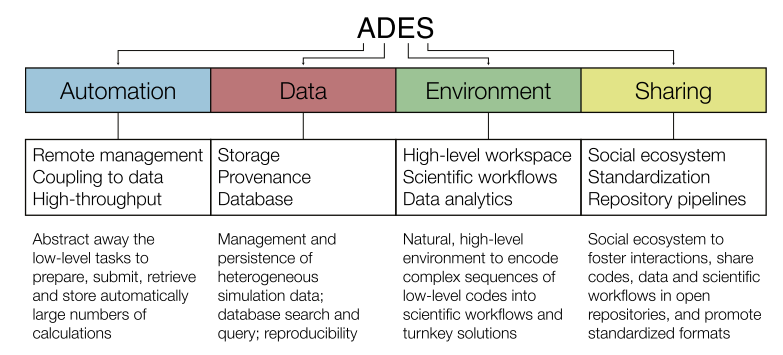
\includegraphics[width=0.86\textwidth]{figs/ch3_ades.png}
  \centering
  \caption{计算科学基础设施工具的四大支柱。在较低的层次上,需要一个自动化框架和一个有效的数据管理解决方案。在用户级别,高级环境与社会生态系统相结合,以促进代码、数据和工作流的共享,图片来源文献\cite{pizzi2016aiida}}
  \label{fig:ch3_ades}
\end{figure}

自动化(A)描述了对底层计算任务参数准备,任务提交,结果检索,计算和数据储存过程封装的自动化过程。从而使AiiDA的用户可以简单快速编写自动化的工作流。a)远端集群管理。大型的计算通常运行在用户工作站,工性能计算集群上。任务作业的准备、提交、任务状态的查询、计算结果的下载往往独立于计算过程本身,用户会频繁地执行这类操作。因此,这类与远端计算资源交互协作的任务在AiiDA中被抽象为特定的用户程序接口(API)并对各种不同的作业调度系统实现特定插件,以自动化作业的管理过程。b)数据的耦合和解耦。为了确保计算的可重复性,数据的储存和自动化流程需要互相耦合,否则,用户在遇见计算流程报错是将会手动尝试解决,而这种人工干预将会使得部分流程无法得到记录,从而丢失数据的完全可重复性,相反的,如果用户在项目中给出了全部的输入,并自动化运行的记录后续全部流程,因其在运行过程中记录数据和数据变化迁移的全部逻辑,就能够确保数据的完全的可重复性。c)高通量计算支持。基于这种自动化的优势,就特定流程的计算,可以变化输入参数,从而对海量的参数进行过滤和扫描以发现最优参数,而这正是高通量计算的主要特征。逐个对海量参数进行运行、分析和过滤是人工难以完成的,借助自动化的工作流可以达到这可目的。

数据(D),涉及计算模拟数据的产生和数据的管理,涵盖以下三个核心方面: a) 存储,即储存高性能计算所产生的大量的异质数据。包含输入参数以及最终结果的文件的自动和永久化存储,以便这些数据在将来能够被引用和分析。另一方面,大部分数据只是临时性的如,检查点等,这类数据可以在模拟结束后丢弃。因此,必须采用依赖于计算代码(这里指使用的材料计算的软件如VASP)所需的的文件存储策略(可由用户定制)来对不同输出文件进行分类。在任何情况下,都应该尽可能记录计算模拟过程中产生的中间文件,这样即使在重新启动后文件被删除时,计算的逻辑流也能被持久化保存。如果确保了计算模拟的可复现性,那么在需要时重新生成中间文件的流程就很简单了。同时,在生成数据的计算代码上存储信息也很重要。如果需要完完全全的再现性,可以参考使用虚拟机或Docker镜像技术来一并储存一模一样的可执行代码。b)可重复性。为了实现工作流的可重复性(或称为复现性),工具流系统需要存储和表示所执行的计算过程本身及其输入数据。然而,一个有效的数据模型不仅应该强调计算和数据,还应该跟踪它们之间的因果关系,即结果的完整来源。例如,对于弛豫后的晶体结构如果不知道它的初始构型,即是如何获得的最后的结构的,这个情况下结果的用途将很有限。我们使用有向无环图作为表示数据和计算之间关系网络的数据结构。c) 数据库。如今常见的计算工作环境通常都由大量具有任意目录结构、任意命名方式和缺乏文档信息的文件组成。在实际应用中,其他用户通常难以清楚地理解和使用这些信息(甚至是数据的创造者自己在一段时间后也对这些数据无能为力),同时大量的混乱的数据也使得很难在存储了许多信息后而还可以容易地检索特定的计算。数据库可以帮助组织和查询结果。上面所说的基于有向无环图的数据模型的实现,不能局限于特定的应用程序,而还必须适应异构数据。它必须能够有效地查询与图形节点相关联的任何属性的信息(包括但不限于数字、字符串、列表、字典等)。另外的,遍历图以评估节点之间因果关系的查询也是必要的。如果满足上述要求,就不需要图形数据库作为后端。例如,AiiDA的后端是一个关系数据库,可用于有效的图遍历。

上面描述的前两个动机主要针对地层的功能。接下来的两大设计动机则是面向用户端的功能实现。其中,环境(E)侧重于为计算科学创造一个社群环境,涉及以下几个方面:a) 具象和可直接使用的工作界面。由于研究人员的目标是进行新的研究发现,而不是应止步于学习新的代码,因此面向用户的基础工具应该灵活且易于使用。例如,尽管数据库在数据驱动的计算科学方面提供了许多优势,但很少有科学家是该方面的专家。因此,数据库管理和连接的复杂性必须通过API抽象层来充分隐藏。此外,通过使用广泛使用的高级编程语言(如AiiDA采用的Python),人们可以受益于各种成熟的以存在的能够用于从数据库插入和检索数据的工具。同时基础工具也必须是模块化的,以提供通用的底层功能核心,以及支持不同计算模拟软件代码的可定制插件的编写。b)科学工作流。许多科学知识不仅存在于最终保存的数据中,还存在于对过程的描述中,即那些用来生成这些数据的“科学工作流程”。如果可以对这些流程进行编码储存,那么就可以在需要的时候重用它们,并用来在不同的情况和条件下计算相似的结果(如仅仅改变流程中的个别参数)。工作流指定了计算步骤之间的依赖关系,依赖关系可能不是在开始时就定义号的的,而是有可能依赖于中间结果(例如,计算材料学中常见的迭代次数未知的迭代收敛)。因此,基础工具应该只有在前面的步骤结束后动态地根据结果生成后续的计算,并在运行时重新生成完整的依赖关系。科学工作流与其他基础涉及动机相配合,帮助用户专注于工作流逻辑,而不是对远程集群的管理使用的细节。一个额外的好处是,在工具执行期间能够自动存储数据来源并提供了一个隐含的有关结果数据逻辑的文档。c)数据分析。应用驱动的计算材料学研究往往需要使用数十种不同的工具和近似方法。然而,用不同代码得到的结果往往都有相同的后处理或可视化算法。这些数据类型(例如晶体结构或带结构)应该以相同的公共格式存储。然后,再通过基础工具来提供数据分析的功能来执行响应的操作,或者充分使用已有的成熟的工具或软件库。这可以通过提供数据处理和分析的外部工具接口来实现(例如晶体结构\cite{ong2013python}),而不需要考虑用于生成数据的具体模拟计算软件代码。

第四个设计动机是共享(S),我们目标创建一个计算材料的生态系统,以促进科学家之间的互动,特别是共享数据、结果共享和科学工作流程共享。a)生态系统。指的是工具的框架应该是一种能够在计算材料研究中能同时创建生态系统的技术,同时需要非常小心地考虑数据访问策略。研究人员有时更喜欢保持他们的数据的私密性(同时保护正在申请的专利或未发表的数据),但如果需要与合作者或公共存储库共享,应该通过很小的努力就可以实现数据保密层级的变化来共享数据。除了数据共享,还应该提供一个标准化的插件接口。使得插件易于编写和设置,用户可以容易地贡献共享工作流,处理新的数据格式,或支持新的计算模拟软件代码。通过这种机制,科学家将能够进行社区型的计算和保证数据共享,这与移动应用程序和网络生态系统的发展并行。b)标准化。为了促进数据交换,研究者之间应商定并采用标准格式来共享数据\cite{murray2003chemical}。即使存在多个不同标准,也可以设想一个可选择的配置,其中每个新计算代码都有以既定格式提供数据。另一方面,定义合适的数据实体也很重要(例如,简化要存储在给定数据库中的物理量的名称和物理单位,以及它们的含义)。特定于领域有其特定的数据实体,其定义必须是社区驱动的(如TCOD\cite{merkys2017posteriori}数据库)。基础工具在这方面将很有用,既可以作为数据实体的生产来源,也可以作为生产包含一组模拟用例的测试环境。c)数据仓库。随着存储仓库的出现,直接导入或导出数据的能力(通过REST接口或通过适当协议)变得很重要。如果建立了格式和数据实体,平台必须简单地将数据及其来源转换为指定的格式。这使得对外部数据库的贡献变得非常简单,同时平台也能成为创建共享存储库的促进者。

\subsection{AiiDA内核的架构设计}

AiiDA在设计上能够广泛适用于各种计算规模的计算科学问题和各种计算能力的计算应用,但其最主要的应用还是对高性能计算(HPC)系统的支持。HPC的用户通常习惯通过脚本来使用计算资源,因此AiiDA的工作流引擎提供了一个丰富的应用软件接口(API)以编写工作流,而非像其他主流工作流管理系统,如Kepler\cite{altintas2004kepler}, Taverna\cite{oinn2004taverna},  和Triana\cite{taylor2003triana},通过提供图形用户接口(GUI)来定制工作流。API能够更加明晰地、无缝地将工作流系统与在高性能计算机上运行的模拟计算代码以及数据处理分析工具结合,从而让用户有最大的自由度来构建符合其目的的合适的工作流。需要说明的是,这种灵活性是以牺牲用户的学习成本实现的,用户需要编写一些简单的脚本,来使用AiiDA构建工作流。但对于已经习惯通过脚本来使用HPC的用户,这样的学习成本非常之小。

基于API的工作流定义方式的另一个优势是,能够定义动态的工作流。动态工作流指的是运行路径并非提前定义并固定的工作流,而是会随着工作流的执行运行时地动态变化执行逻辑的工作流。最显而易见的例子是计算流程的错误处理与恢复。在AiiDA中,定义工作流的代码是被其引擎直接运行,而不通过中间层,这点与多数工作流管理系统区别,它们通过静态的标记语言如XML或通用工作流语言(CWL)\cite{amstutz2016common}来定义工作流,然后转化为无环图(DAG)的形式以供运行。静态工作流的最大劣势也就是动态工作流的最大优势,就是整个工作流的运行步骤是不需要提前确定的,这使得编写有程序逻辑的工作流成为可能。

AiiDA的软件架构理论上很好的反映了针对高通量计算材料学所追求的目标。包括运行设备的可拓展性,即可以在小型个人电脑上运行也能在高性能计算集群上运行以及可以运行各种时间范围的任务,小到仅需几秒钟完成的小型处理型任务,大到需要几周时间完成的运行在高性能集群上的任务。另外,它能在一个设备上同时处理成千上万这样的进程。开发中时,AiiDA被设计为安装运行在用户的个人工作站上,但在实际生产环境中AiiDA可以被一群人通过多用户的方式一起使用,甚至能够运行在如Material Cloud\cite{talirz2020materials}这样的公共平台上。

如图\ref{fig:client-worker}所示,工作流引擎依赖使用以下两个外部组建来运行工作流:a)数据库引擎(PostgreSQL\cite{postgresql}),用于保存每个进程的当前运行状态。并且该数据库还充当了向用户展示进程运行状态的功能。b)消息中间件组建(RabbitMQ\cite{rabbitmq})用于在客户端和服务端之间传输有关进程状态的消息。该组建即可以运行在AiiDA内核所运行的机器上,也能运行在独立的一个服务器上。通过这样层级的解耦,开发中和使用时的效率被大大提升。

\begin{figure}
  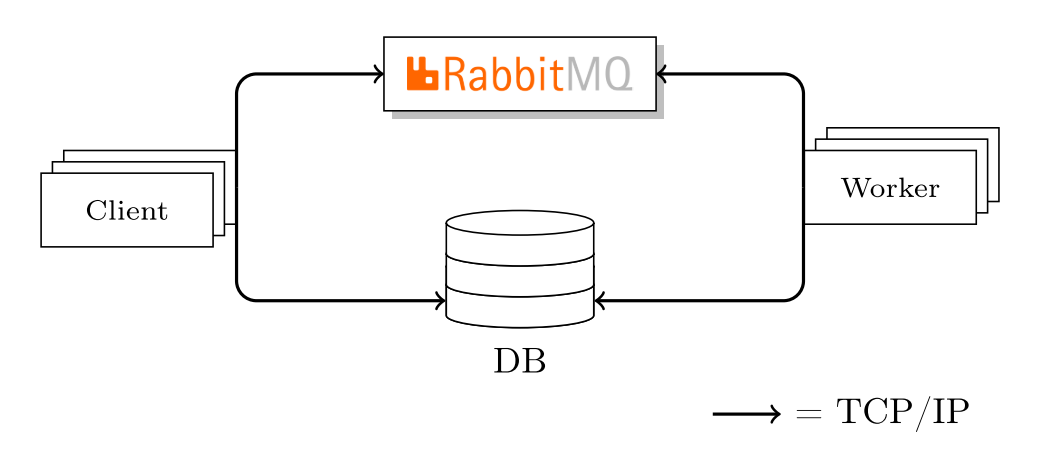
\includegraphics[width=0.92\textwidth]{figs/db-rmq.png}
  \caption{客户端和运行端通过TCP/IP连接到数据库和RabbitMQ服务,支持丰富的可能配置和相应的使用场景。守护进程在一个单独的Python进程(称为worker)中管理多个并发的运行程序。每个运行器串行执行,但仍然能够在使用Python协程等待进程时通过切换槽来处理多个AiiDA进程。}
  \label{fig:client-worker}
\end{figure}

为了能够设计上工作流系统响应性、可拓展性、支持高通量的目标,我们极大的依赖于通过事件触发作为进程运行中的进程控制信号。比如当一个工作流在运行中等待远端完成任务时,或者当向运行的进程发送一个终止信号后等待其完全关闭的过程中,所有的进程的状态转换都是通过进程相关的状态机的事件来触发的。这种涉及和基于等待队列的系统形成对比,等待队列的系统拥有一个管理进程的池,在进程运行时通过不断的查询进程状态来改变和触发后续要执行的动作。这种系统在高性能集群的任务调度系统中使用较多,因为集群上的任务往往都有较长的运行时间。但这种进程管理的触发后续任务的方式的响应性较低,不符合我们在运行高通量计算处理快速进程时要求快速响应的特点。

与其他的基于事件的系统如用户界面系统、计算机游戏等类似,AiiDA使用事件循环来实现这一目标,我们选择使用asyncio这一Python自带的库来实现这一目的。这使得多个AiiDA进程可以通过一个单独的Python进程进行管理,尽管没有多线程的支持异步运行的协程之间还是能够合理的被调度和运行,在等待外部设备读写的过程中可以快速地将计算机进程的使用权交由其他协程来处理。使用协程而非线程技术来处理多任务的共同运行还解决了数据库读写的负载问题,因为默认的数据库服务器的连接数通常不多,如PostgreSQL默认仅支持100个连接。而且,使用多线程来编程非常的反直觉并且难以开发调试,即便是对于经验丰富的程序员针对多线程的开发调试也是非常困难的,特别是在AiiDA中我们对如何调用API没有施加过多的特殊限制。

执行工作流所需的全部Python组件都集中在\texttt{Runner}类中,该类提供事件循环、状态记录、传输(例如SSH)以及一些其他功能,其中一些功能将在下面进行更详细的描述。由于使用了事件循环,每个运行器(Runner)可以并发地运行内存限制内任意数量的工作流进程。我们把可以在单个运行程序上运行的进程数称为任务槽数。

运行器可以在本地终端中独立使用。但在大多数生产环境中,用户希望启动一个可以管理一个或多个运行程序的守护进程,同时支持在运行程序崩溃时通过守护进程自动重新启动。在AiiDA中,我们使用Circus库\cite{circus}来实现这一功能。Circus提供了启动多个运行系统进程的功能,当运行的进程崩溃时,Circus会记录并按照用户定制的方式自动重新启动终断的进程。此外,它还可以显示有关进程运行所需要的当前资源使用情况的信息,并可以支持动态增加运行时池中运行的系统进程的数量。

\begin{figure}
    \centering
\begin{tikzpicture}[auto]

\begin{groupplot}[
    group style={
        group size=2 by 1,
        xticklabels at=edge bottom,
        horizontal sep=0pt
    },
    axis lines = left,
    ylabel = {\# slots},
    ymin=0, ymax=5,
    xmin=0, xmax=101,
    ytick={0, 1, 2, 3, 4, 5},
    yticklabels = {0, 1, 2, 3, 4, $\ldots$},
    scale only axis,
]
\tikzstyle{cell} = [execute at begin node=\scriptsize, text centered, anchor=center]
\nextgroupplot[
    xmin=0,xmax=4,
    ymin=0,ymax=5,
    width=4cm,
    height=5cm,
    xlabel = {\# workers},
]
\draw (axis cs: 0,0) rectangle node[cell] {W0-S0} (axis cs: 1,1);
\draw (axis cs: 0,1) rectangle node[cell] (w1s2) {W0-S1} (axis cs: 1,2);
\draw[color=black!70] (axis cs: 0,2) rectangle node[anchor=center] (w1s3) {} (axis cs: 1,3);
\draw[color=black!40] (axis cs: 0,3) rectangle (axis cs: 1,4);
\draw[color=black!10] (axis cs: 0,4) rectangle (axis cs: 1,5);

\draw (axis cs: 1,0) rectangle node[cell] (w1s0) {W1-S0} (axis cs: 2,1);
\draw (axis cs: 1,1) rectangle node[cell] {W1-S1} (axis cs: 2,2);
\draw[color=black!70] (axis cs: 1,2) rectangle (axis cs: 2,3);
\draw[color=black!40] (axis cs: 1,3) rectangle (axis cs: 2,4);
\draw[color=black!10] (axis cs: 1,4) rectangle (axis cs: 2,5);

\draw[color=black!70] (axis cs: 2,0) rectangle node[anchor=center] (w3s1) {} (axis cs: 3,1);
\draw[color=black!70] (axis cs: 2,1) rectangle (axis cs: 3,2);
\draw[color=black!70] (axis cs: 2,2) rectangle (axis cs: 3,3);
\draw[color=black!40] (axis cs: 2,3) rectangle (axis cs: 3,4);
\draw[color=black!10] (axis cs: 2,4) rectangle (axis cs: 3,5);

\draw[color=black!40] (axis cs: 3,0) rectangle (axis cs: 4,1);
\draw[color=black!40] (axis cs: 3,1) rectangle (axis cs: 4,2);
\draw[color=black!40] (axis cs: 3,2) rectangle (axis cs: 4,3);
\draw[color=black!40] (axis cs: 3,3) rectangle (axis cs: 4,4);
\draw[color=black!10] (axis cs: 3,4) rectangle (axis cs: 4,5);

\draw[color=black!10] (axis cs: 4,0) rectangle (axis cs: 5,1);
\draw[color=black!10] (axis cs: 4,1) rectangle (axis cs: 5,2);
\draw[color=black!10] (axis cs: 4,2) rectangle (axis cs: 5,3);
\draw[color=black!10] (axis cs: 4,3) rectangle (axis cs: 5,4);
\draw[color=black!10] (axis cs: 4,4) rectangle (axis cs: 5,5);

\draw[->] (w1s0) -- (w3s1);
\draw[->] (w1s2) -- (w1s3);

\nextgroupplot[
    xmin=99, xmax=101,
    ymin=0, ymax=5,
    xtick = {99,100,101},
    xticklabels={,$\ldots$,},
    axis y line=none,
    axis x line=middle,
    axis x discontinuity=crunch,
    height=5cm,
    width=2cm
]

\draw[color=black!10] (axis cs: 99,1) rectangle (axis cs: 100,2);
\draw[color=black!10] (axis cs: 99,2) rectangle (axis cs: 100,3);
\draw[color=black!10] (axis cs: 99,3) rectangle (axis cs: 100,4);
\draw[color=black!10] (axis cs: 99,4) rectangle (axis cs: 100,5);

\draw (axis cs:100,0) -- (axis cs:100,6);
\node[rotate=90,fill=white,anchor=center] at (axis cs:100,2.5) {Max. connections};

\end{groupplot}

\node[anchor=south west, xshift=-12pt,fill=white,fill opacity=0.8,text opacity=1] at (w1s3) {\small Vertical scaling};
\node[anchor=west,fill=white,fill opacity=0.8,text opacity=1] at (w3s1) {\small Horizontal scaling};


\end{tikzpicture}
    \caption{
    每个runner中worker的数量和插槽数量的变化范围。可接受的并发的AiiDA过程的总数是两个坐标轴上的值的乘积
    }
    \label{fig:daemon-scaling}
\end{figure}


使用这个守护进程,如图\ref{fig:daemon-scaling}所示,你可以垂直扩展(每个runner有多个插槽)和水平扩展(多个Python实例,每个实例有一个runner)。对于需要大量python内处理的工作负载,最好在工作时扩展worker的数量——涉及许多远程计算的负载可以扩展每个worker的插槽数量,从而实现在运行守护进程的计算机上最小化负载系统资源减,少吞吐量的损失。当worker的数量等于数据库连接的最大数量时,就达到了限制上限,用户无法再增加运行对象,但如果用户能够访问数据库设置,那么这个数据库相关的上限是可配置的。

AiiDA工作流引擎运行时的主要工作对象是\texttt{Process}类。所有其他类如\texttt{WorkChaian}类、\texttt{CalcJobs}类等)都是从\texttt{Process}(或其子类)派生而来的,因此继承了大量原始类的常见功能和特性。\texttt{Process}类本身是为一个扩展的状态机,这意味着由一个有限状态机组成,如图\ref{fig:process_state_machine}所示,其中每个状态都可以有内部数据作为其扩展状态的一部分。这是事件驱动系统中常见的模式,因为它提供了统一的方式来定制特定状态,以及触发事件的动作,这些事件触发动作(hook)可以用作触发器,在状态转换期间执行流程特定的内部逻辑或外部数据交换等操作。事件触发动作本身以\texttt{Process}类的成员函数形式定义,比如:

\begin{lstlisting}[
    language=python,
    label=code:state-transition-hooks,
    caption={AiiDA's \texttt{Process} state transition hooks.
    These are invaluable for being able to guarantee that certain actions are performed when a state transition occurs.},
]
# Entering a new state
def on_entering(self, state):
    ...

# Just entered the new state from 'from_state'
def on_entered(self, from_state):
    ...

# About to exit the current state
def on_exiting(self):
    ...
\end{lstlisting}

通过使用这些事件触发器,可以有选择地在状态转换的不同时刻执行相应的动作,如上面例子中,\texttt{on\_entered}触发后保证了完成后的状态一致。这些触发器在AiiDA中的一个重要用途是,它能够将进程的当前状态反射回数据库,同时包括了记录和保存当前进程的检查点状态及信息。状态转换触发器还可以用于发送广播消息,允许接受客户端(可能位于远程机器上)在当前进程状态更改时更新它们在数据库中的状态信息。

\begin{figure}
\center
\begin{tikzpicture}[>=stealth',shorten >=1pt,auto]
%                   ___
%                  |   v
%     CREATED --- RUNNING --- FINISHED (o)
%                  |   ^     /
%                  v   |    /
%                  WAITING--
%                  |   ^
%                   ----


%       * -- EXCEPTED (o)
%       * -- KILLED (o)
    \tikzstyle{every state}=[node distance=2.5cm, font=\tiny, minimum size=16pt]
    \node[state,initial,label=above:{Created}] (created) {};
    \node[state,right of=created, label=above right:{Running}] (running) {};
    % Terminal states
    \node[state,accepting,right of=running, label=below:{Finished}] (finished) {};
    \node[state,accepting,below of=created, label=below:{Excepted}] (excepted) {};
    \node[state,accepting,below of=running, label=left:{Killed}] (killed) {};

    \node[state,below of=finished, label=below:{Waiting}] (waiting) {};


    \path[->] (created) edge (running)
              (running) edge (finished)
              (running) edge [loop above] (running)
              (running) edge [bend right=15] (waiting)
              (waiting) edge [bend right=15.] (running);

    \path[->] (created) edge (killed);
    \path[->] (running) edge (killed);
    \path[->] (waiting) edge (killed);

    \path[->] (created) edge (excepted);
    \path[->] (running) edge (excepted);
    \path[->] (waiting) edge[bend left] (excepted);
\end{tikzpicture}
\caption{
  进程状态机。
  终止状态用一个双环表示。
}
\label{fig:process_state_machine}
\end{figure}

一个完整的进程通常会经过各种状态,可能在状态转移时分别运行几个成员函数或等待其他进程完成。但是,如果进程中发生异常,则该异常会被捕获,运行器(Runner)将会把进程转换到终端例外状态,并同时创建一个日志条目,以包括对Python堆栈信息的跟踪。而另一种手动使进程提前终止的方法是调用\texttt{kill}成员方法,来使进程进入终止状态。

引擎在实现中的一个重要设计是,进程的运行是具有检查点和可以被持久化保存的的。这样,在有意或无意关闭进程的情况下,AiiDA可以在引擎重新启动后从最后的被保存的正确运行时状态恢复并继续运行,从而实现了计算机的关闭(断电或人为关机)不会影响长时间的任务进程的良好运行。为了实现这一点,我们使用了在进程状态转换时将检查点及相应进程信息写入数据库。具体来说,任务进程的相关上下文信息、输出和特定的元数据将会被保存到一个字典数据结构中,然后由AiiDA构建特定的持久化保存的数据结构存入数据库中,整个检查点的持久化储存的方式如图\ref{fig:persister}所示。

\begin{figure}
  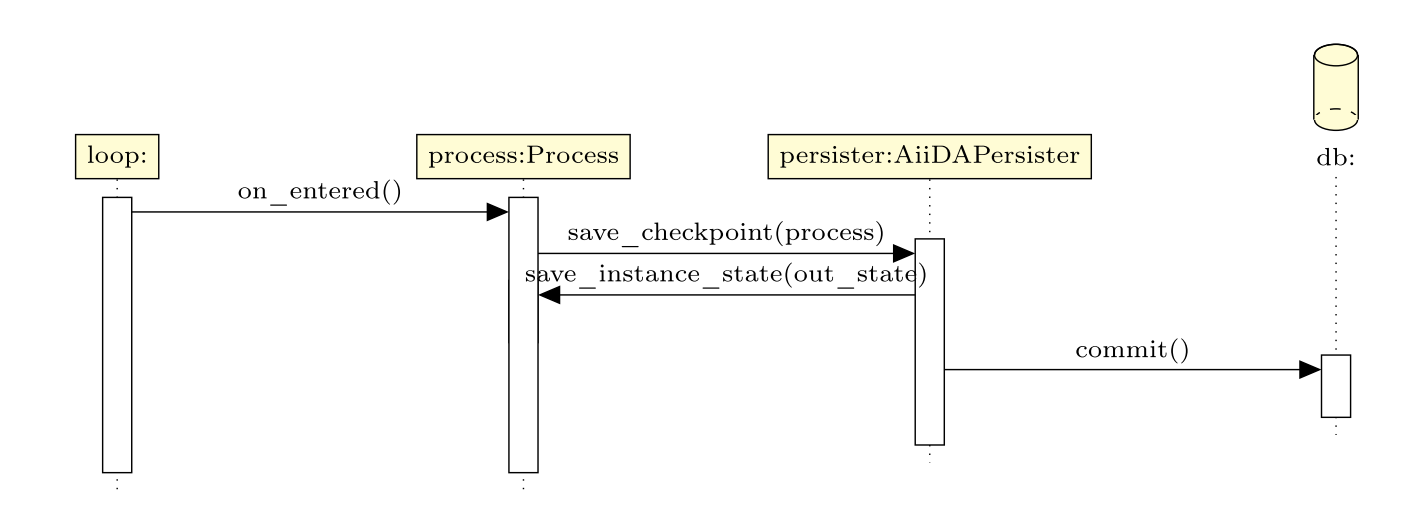
\includegraphics[width=0.96\textwidth]{figs/persister.png}
  \centering
  \caption{显示在状态转换时流程的内部状态的持久性的UML活动图。竖条显示实体(顶部)活动期间的时间,因此定义了它的范围。当持久化进程获得保存检查点的请求时,它调用进程并请求它生成一个字典,即\texttt{out\_state},然后将其序列化并提交给数据库}
  \label{fig:persister}
\end{figure}

工作流引擎主要通过消息传递来对流程进行外部控制,并以此在确保容错的同时保持高吞吐量。而消息传递是通过使用被称为消息中间件的组件实现的,在我们的例子中使用了RabbitMQ这一开源的消息中间件组件。消息中间件通常负责保证消息的持久性和独立性,通过与应用程序内部逻辑解耦来使应用程序内部仅关注其相应的业务逻辑。在RabbitMQ中,用户需要首先在服务端安装并打开一个消息传递服务,再使用客户端软件通过TCP端口进行消息交互。消息的路由和信息持久化保存均是由RabbitMQ内部处理实现的,这大大简化了我们开发的工作量。

为了方便AiiDA与RabbitMQ交互,我们开发了一个Python库kiwiPy, kiwiPy依赖\texttt{aio\_pika}库实现和RabbitMQ的交互。KiwiPy最大可能模拟并封装了与RabbitMQ的主要交互过程,并提供了将通信信息装在到单独线程的功能。这中封装对于AiiDA来说至关重要,详细信息请参考接下来的有关任务队列的小节。同时,除了任务队列外,kiwiPy还为AiiDA提供发送远程函数调用(RPC)和广播消息的能力。

任务队列用于安排和调度要运行的新进程。使用RabbitMQ的一个主要的优势时它能够根据所选择的设置提供了一定的消息成功传输的保证。对于我们的任务队列,AiiDA使用持久化的消息,这些消息被持久化保存到磁盘中,以便在机器有意或无意地重新启动后仍然存在并可以恢复到机器关闭前的状态。因此,作业一旦从客户机交付给代理,就需要确保永远不会丢失。此外,RabbitMQ还需要知晓已经完成的任务,因为如果它失去了与worker的连接,它会自动重新将任务排到队列中,直到确认任务执行完成。这种机制依赖于周期消息这一组件,一般也被称为心跳包, worker必须在设定的时间周期内及时作出响应,否则,当连续两个心跳包响应丢失时,RabbitMQ会认为worker已经中止运行,并触发重调度机制。也是因为这个原因,kiwiPy额外地运行在一个独立的线程中(与其他真实的任务独立),以此确保即使AiiDA进程在一个有极大的阻塞的工作负载下,它也能够正常地响应心跳。

RPC全称为Remote Procedure Call即远程函数调用。正如其名称所暗示的,这些类型的消息用于调用特定过程(在我们的例子中是函数或类的方法),并将过程的结果传递回给调用者。这主要用于暂停、执行和终止特定的活动进程。

广播功能涉及到向任意以定义的侦听器发送单个消息,它们不需要收到特定的响应。该模式主要有两个目的,分别是暂停、执行或终止包含多个进程的进程组,并控制它们之间的信息流。已经产生子进程的父进程可以选择等待子进程完成后再继续执行。父进程通过将自己注册定义为子进程广播的监听器,当它接收到子进程终止消息时,父进程可以方便地实现对进程终止。这种机制使AiiDA中\texttt{to\_context}的工作链构造的功能得以实现,即当工作链中的进程可以通知工作链当它所等待的流程完成时该进程可以继续进行。
